\documentclass[12pt,twoside]{article}

\def\refname{\underline{\normalsize References}}
\def\title#1{\begin{center}{\large\bf #1}\end{center}}

\renewcommand{\author}[2]{\noindent\underbar{#1}\\#2\\}
\newcommand{\coauthor}[2]{\noindent\underbar{#1}\\#2\\}

\usepackage[paperwidth=20.5cm,paperheight=29.7cm,width=18cm,height=26.5cm,top=24mm,left=14mm,headsep=11mm]{geometry}

\usepackage{graphicx}

\usepackage{amsmath,bm}

\pagestyle{myheadings} \markboth{DAYS on DIFFRACTION 2016}{DAYS on DIFFRACTION 2016}

\begin{document}

\title{Resonant states for quantum ring with two infinite leads}

\author{\textbf{Gerasimov D.A.}, Popov I.Yu., Popov A.I.} % presenting author is marked out by \textbf 
{Department of Higher Mathematics, ITMO University, Saint Petersburg 197101,
Russia\\ e-mail: {\tt karlicoss@gmail.com, popov1955@gmail.com, popov239@gmail.com} }

% for name index
\index{Gerasimov, D.A.} 
\index{Popov, I.Yu.}
\index{Popov, A.I.}

\newcommand\abs[1]{\left|#1\right|}

Quantum graph is a widely used model of nanosystem [1-4]. If the graph $\Gamma$ consists of finite number of edges of finite lengths, then the Hamiltonian has purely discrete spectrum and the eigenfunctions are complete in $L_2(\Gamma)$. If $\Gamma$ contains semi-infinite edges, one has non-empty continuous spectrum and resonances generated by the eigenvalues of the Hamiltonian of finite graph. For many applications, it is important to know a space in which the resonant states form a complete system. In this paper we determine this space for a graph with two infinite leads and a loop (Fig.~1) using Sz.-Nagy model [5].

\medskip
\centerline{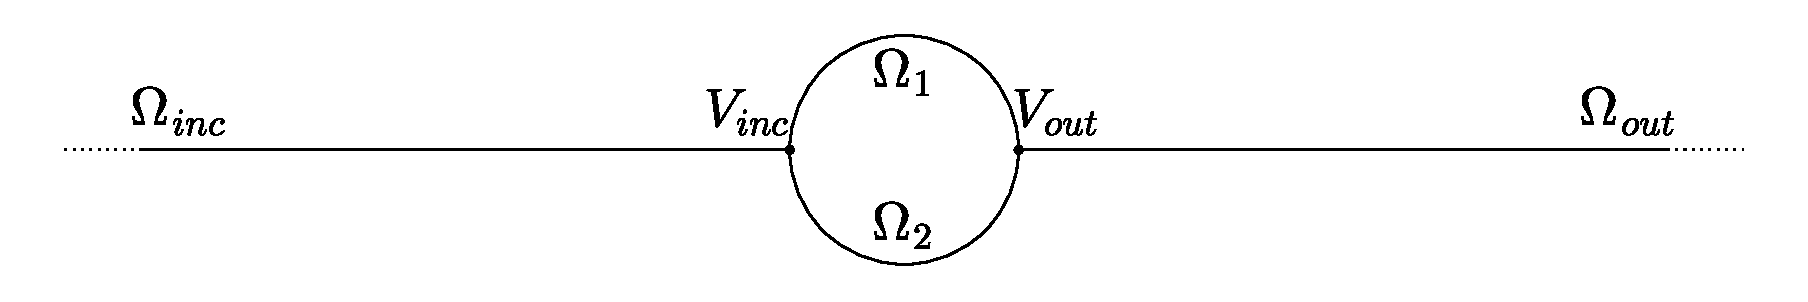
\includegraphics[width=120mm]{graph.eps}}
\medskip
{\narrower\noindent \textbf{Fig.~1:}
Quantum graph $\Gamma$ consisting of edges $\Omega_{inc}, \Omega_{out}, \Omega_1, \Omega_2$. $\Omega_1$ and $\Omega_2$ represent the 1D ring connected to lead $\Omega_{inc}$ via the vertex $V_{inc}$ and to lead $\Omega_{out}$ via $V_{out}$.
\par}
\medskip
% $-\psi'_{inc}(V_{inc}) + \psi_1'(V_{inc}) + \psi_2'(V_{inc}) = a \psi_{inc}(V_{inc})$; $\psi'_{out}(V_{out}) - \psi_1'(V_{out}) - \psi_2'(V_{out}) = a \psi_{out}(V_{out}) $
We are interested in scattering of a wave with wavevector $k$ incoming from the left lead to the right one. At vertices $V_{inc}, V_{out}$ we impose Dirichlet boundary conditions for wavefunctions and $\delta$-coupling boundary conditions with the coupling constant $a$ for wavefunction's derivative.
After solving the system of equations, we obtain a closed-form expression for the S-matrix determinant:
\[
\det S = \frac{((a^2 - 5k^2) \cos(kd) \sin(kd) -4ak \sin^2(kd) + 2ak) + i (2ak \cos(kd) \sin(kd) -4k^2 \sin^2(kd) + 2k^2)}{((a^2 - 5k^2) \cos(kd) \sin(kd) -4ak \sin^2(kd) + 2ak) - i (2ak \cos(kd) \sin(kd) -4k^2 \sin^2(kd) + 2k^2)}
\]

To establish the completeness, we have to prove that $S$ is a Blaschke-Potapov product [6], that is, $\lim\limits_{r \to 1 - 0} \int\limits_{L_r} \log  \abs{\det S(k)} \frac{dk}{(k - 1)^2} = 0$, where $L_r$ is the image of the curve $\abs{\xi} = r$ ($r < 1$) under the map $k = i \frac{1 + \xi}{1 - \xi}$. Substituting $\det S$, which we calculated above, and estimating the integral, one obtains the desired result.

This work was partially financially supported by the Government of the Russian Federation (grant 074-U01), by Ministry of Science and Education of the Russian Federation (GOSZADANIE 2014/190, Projects No 14.Z50.31.0031 and No. 1.754.2014/K), by grant MK-5001.2015.1 of the President of the Russian Federation and DFG Grant NE~1439/3-1.

\begin{thebibliography}{9}

\bibitem{1} P.Kuchment, \textit{Waves in Random Media}, \textbf{12}(4), R1-R24 (2002)

\bibitem{2} I.S. Lobanov, A.I. Trifanov, E.S. Trifanova, \textit{Nanosystems: Phys. Chem. Math.}, \textbf{3}(4), 512-523 (2013).

\bibitem{3} P.Exter. J.P. Keating, P. Kuchment, T. Sunada, A. Teplyaev (eds.), \textit{Analysis on Graphs and Its Applications}. Proc. Symp. Pure Math., 77 (Providence, RI: Amer. Math. Soc.) (2008)

\bibitem{4} I.Yu. Popov, A.N. Skorydina, I.V. Blinova, \textit{J. Math. Phys.}, \textbf{55}, 033504 (2014)

\bibitem{5} B. Sz.-Nagy, C. Foias, H. Bercoviuci, L. Kerchy, \textit{Harmonic Analysis of Operators on Hilbert Space}, 2nd edition, Berlin: Springer (2010)

\bibitem{6} N.K. Nikolskii, \textit{Tretise on the Shift Operator}, Berlin: Springer (1986) 

\end{thebibliography}

\end{document}
